\documentclass[11pt]{beamer}
\title{Polynomial Invariant Generation for Non-deterministic  Recursive Program}
\usepackage{verbatim}
\usepackage{amsmath}
\usepackage{amsthm}
\usepackage{listings}
\usepackage{graphics}
\usepackage{color}
\usepackage{multicol}
\usepackage{stmaryrd}\usefonttheme[onlymath]{serif}

\newtheorem{proposition}{Proposition}
\author{Krishnendu Chatterjee et al.}
\date{\today}


\begin{document}
\maketitle

\begin{frame}\frametitle{Problem}

Invariant generation:
\begin{itemize}
\item Program: programs with \textbf{polynomial assignments}.


\item Invariant: conjunction of strict \textbf{polynomial inequalities}.
\end{itemize}

Find a sound and complete algorithm for the synthesis.


\end{frame}

\begin{frame}\frametitle{Contributions}

\begin{itemize}
\item Non-recursive: A sound and complete method to generate polynomial invariants for polynomial programs (template-based).
\item The method can be extended to handle recursion.
\item Worst-case complexity: subexponential.
\item Weak invariant: can be reduced to solving a quadratically-constrained linear program (QCLP).
\end{itemize}
\end{frame}

\begin{frame}\frametitle{Contribution: Comparison}
\begin{center}
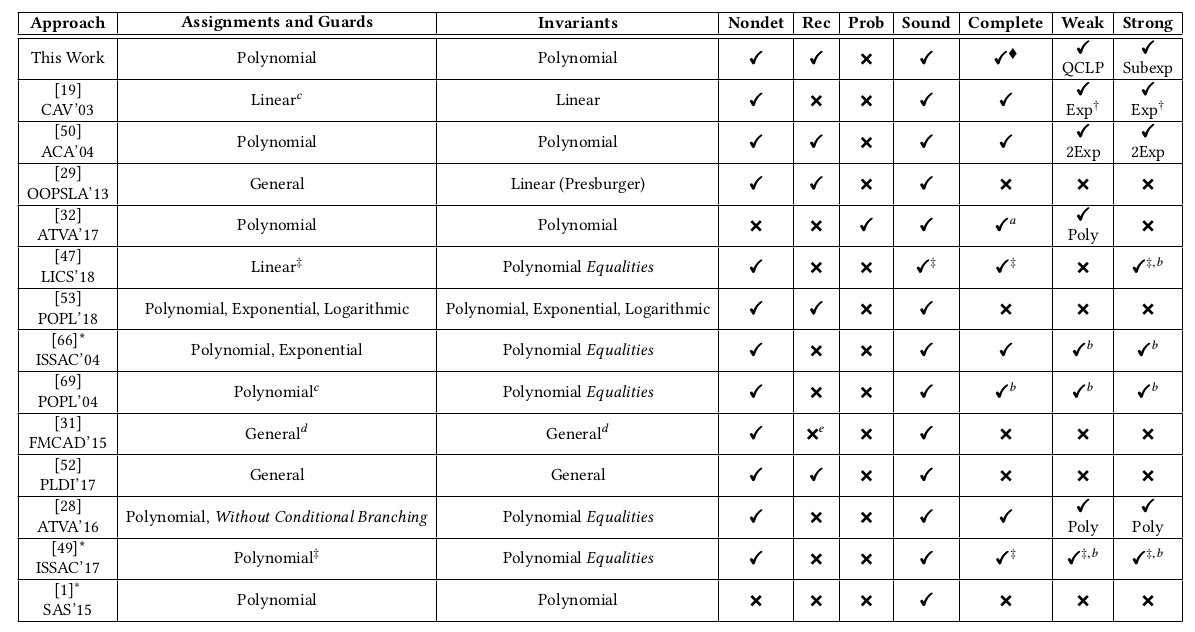
\includegraphics[scale=0.26]{table.png}
\end{center}
\end{frame}

\begin{frame}\frametitle{Overview}

\begin{itemize}

\item A demo example.
\item Algorithm.
\begin{enumerate}

\item Computation model.
\item Preliminaries: program, invariant and mathmatical tools.
\item Algorithm for non-recursive programs.
\item Soundness and semi-completeness.
\item Algorithm for recursive program.

\end{enumerate}

\item Experimental Results.
\end{itemize}

\end{frame}


\begin{frame}\frametitle{Example: Basic Idea}
Goal: synthesize a postcondition and invariants. 
\begin{center}
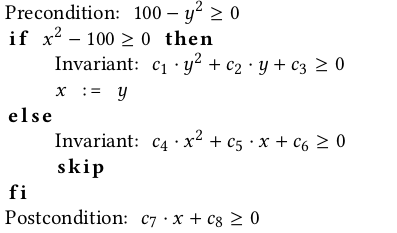
\includegraphics[scale=0.4]{example1.png}
\end{center}

\[100-y^2 \ge 0 \wedge x^2 - 100\ge 0 \Rightarrow c_1y^2 + c_2y+c_3\ge 0\]
\[100-y^2 \ge 0 \wedge x^2 - 100\ge 0 \Rightarrow c_4x^2+ c_5x+c_6< 0\]
\[c_1y^2 + c_2y+c_3\ge 0\Rightarrow c_7y + c_8 \ge 0\]
\[c_4x^2+ c_5x+c_6\ge 0\Rightarrow c_7x + c_8 \ge 0\]

\end{frame}

\begin{frame}\frametitle{Example: Basic Idea}
\begin{center}
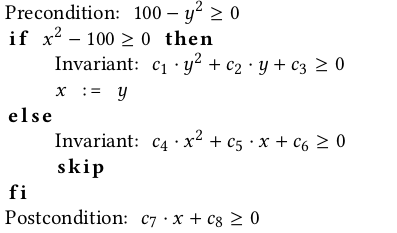
\includegraphics[scale=0.3]{example1.png}
\end{center}
\begin{footnotesize}

\[100-y^2 \ge 0 \wedge x^2 - 100\ge 0 \Rightarrow c_1y^2 + c_2y+c_3\ge 0\]
\[100-y^2 \ge 0 \wedge x^2 - 100\ge 0 \Rightarrow c_4x^2+ c_5x+c_6< 0\]
\end{footnotesize}
Directly: $c_1 = -1, c_2 = 0, c_3 = 100$, $c_4 = 1, c_5 = 0, c_6 = 100$.

\[c_1y^2 + c_2y+c_3\ge 0\Rightarrow c_7y + c_8 \ge 0\]

\end{frame}
\begin{frame}\frametitle{Example: Basic Idea}
\begin{small}
\[c_1y^2 + c_2y+c_3\ge 0\Rightarrow c_7y + c_8 \ge 0\]
\end{small}

\begin{enumerate}
\item wlog. We can add tautology to assumptions.
\begin{small}
\[c_1y^2 + c_2y+c_3\ge 0 \wedge (ay - b)^2\ge 0\Rightarrow c_7y + c_8 \ge 0\]
\end{small}
\item Expanded: 
\[c_7y + c_8 = (ay - b)^2 + d(c_1y^2 + c_2y + c_3)\]

\item Parameters are equal:
\begin{multicols}{2}
$0 = a^2 + c_1d$

$c_7 = -2ab + c_2d$

$c_8 = b^2 + c_3d$

$ .$

With previous valuation for $c_1,c_2,c_3$ and put into  we have 

$c_7 = -1, c_8 = 10, $

$a = \frac{1}{2\sqrt{5}}, b = \sqrt{5}, d = \frac{1}{20}$

\end{multicols}

\end{enumerate}

\end{frame}


\begin{frame}\frametitle{Example: General}
\begin{itemize}
\item \textbf{Soundness}:
To prove 
\[g_1\ge 0, g_2\ge 0, \ldots, g_m \ge 0 \Rightarrow g \ge 0\]
where $g, g_i's$ are polynomials.

\[g = h_0 + \sum_{i = 1}^m h_i\cdot g_i\]
where $h_i$ is sum of squares.

\item \textbf{Semi-completeness}:
In real algebraic geometry: Putinar's Positivstellensatz Theorem.

\end{itemize}


\end{frame}


\begin{frame}\frametitle{Preliminaries: Program}

\begin{example}
\begin{multicols}{2}

\begin{center}
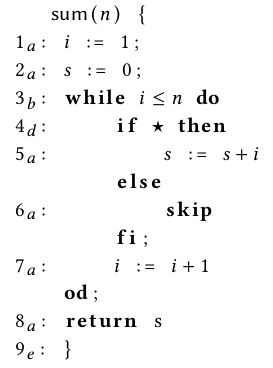
\includegraphics[scale=0.4]{example2.png}
\end{center}

\begin{itemize}

\item Sets of labels: $\mathbf{L}_a, \mathbf{L}_b, \mathbf{L}_c, \mathbf{L}_d, \mathbf{L}_e$

\item Set of variables: 

$V_*^f = \{\texttt{ret}^f, n, \bar{n}\}$

$V^f =V_*^f \cup \{s, i\}$

\item 
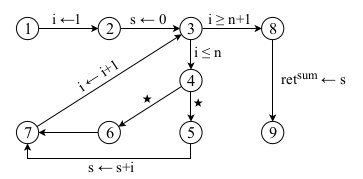
\includegraphics[scale=0.4]{example2cfg.png}

\end{itemize}

\end{multicols}

\end{example}
\end{frame}

\begin{frame}\frametitle{Preliminaries: Invariants}
In the following $\mathfrak{e}$s' are all arithmetic expressions.
\begin{itemize}
\item Pre-conditions: $\texttt{Pre}(l) = \bigwedge_{i = 1}^m \mathfrak{e}_i \ge 0$ over $V^f$.
\item Post-conditions: $\texttt{Post}(f) = \bigwedge_{i = 1}^m \mathfrak{e}_i > 0$ over input variables and return variable.
\item Invariants: $\texttt{Inv}(l) = \bigwedge_{i = 1}^m \mathfrak{e}_i > 0$ over $V^f$.
\item Inductive invariants: Initialization($\texttt{Pre}(l_{in})\Rightarrow \texttt{Ind}(l_{in})$)  and Consecution.
\item Abstract Path: use pre- and post- conditions  as a behavior of a function.

\item Recursive inductive invariants:  initiation, consecution and post-condition consecution.
\end{itemize}


\end{frame}	

\begin{frame}\frametitle{Preliminaries: Theorems}
\begin{theorem}[Putinar's Positivstellensatz]
$g_1, \ldots, g_m, g \in \mathbb{R}[V]$ are polynomials over $V$ with real coefficients. 

 Let $\Pi := \{x\in \mathbb{R}^{V}\mid \forall i. g_i(x) \ge 0\}$.
 If 
 \begin{itemize}
 \item  $\{x\in \mathbb{R}^{V}\mid g_k(x) \ge 0\}$ is compact.
 \item $g(x) > 0$ for all $x\in \Pi$.
 \end{itemize}
 then,
 \[g = h_0 + \sum_{i = 1}^m h_i\cdot g_i\]

\end{theorem}

\begin{lemma}
Given a $h\in \mathbb{R}[V]$, deciding whether $h = \Sigma_i f_i^2$ can be reduced in polynomial time to solving a system of quadratic equalities.

\end{lemma}
\end{frame}

\begin{frame}\frametitle{Algorithm: Non-recursive}

\textbf{Input:} Program $P$, polynomial precondition \texttt{Pre}, max polynomial degree $d$, max size for invariant $n$ and a parameter $\gamma$

\textbf{Step 1:} Setting up templates.
\begin{center}
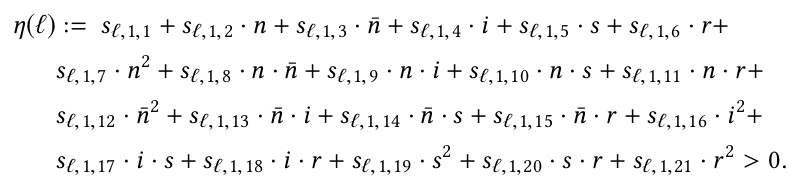
\includegraphics[scale=0.3]{template2.png}
\end{center}
\textbf{Step 2:} Setting up constraint pairs for each transition in CFG.

$(\Gamma, g)$. where $\Gamma = \bigwedge_{i = 1}^m g_i \ge 0$. 


\textbf{Step 3:} Translating constraint pairs to quadratic equalities.

For each pair above, compute the equation of the form
\begin{center}
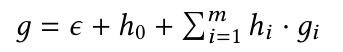
\includegraphics[scale=0.4]{equation1.png}
\end{center}
where $h_i = \Sigma_{j = 1}^rh_i\cdot m_j'$, and $m_j'$ is monomial of degree at most $\lambda$.

\textbf{Step 4:} Finding representative solutions for quadratic equalities from above coefficients equal.

\end{frame}

\begin{frame}\frametitle{Algorithm: Complexity}
\begin{itemize}

\item During the algorithm above, the system's size is polynomially dependent on number of lines of the program (for each transition in CFG).

\item Solving the quadratic inequalities system is in subexponential time.
\end{itemize}

\begin{theorem}[Strong Invariant Synthesis]
Given a non-recursive program $P$ and a precondition that satisfy the compactness condition, above algorithm solves the strong invariant synthesis problem in subexponential time. The solution is sound and semi-complete.
\end{theorem}


\end{frame}

\begin{frame}\frametitle{Recursive Program}
Differences:

\begin{itemize}
\item \textbf{Step 1}: add setting up templates for post-conditions of functions.

\item \textbf{Step 2}: 

setting up constraints pairs for function-call statements and post-condition consecution.

\end{itemize}



\end{frame}

\begin{frame}\frametitle{Implementation and Experimental Results}

\begin{small}

Implemented in Java. 
QCLP Solver: LOQO.

Parameter $\gamma$: highest degree of the input program.

Non-recursive: 
\begin{center}
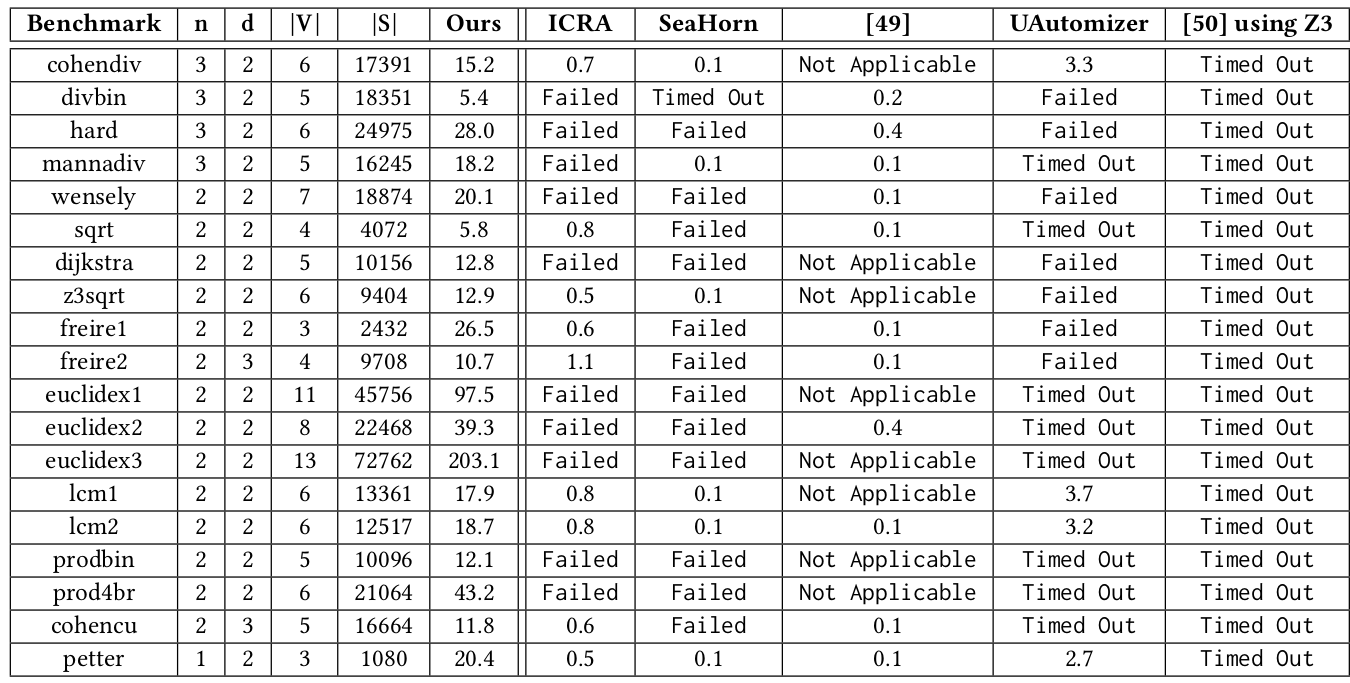
\includegraphics[scale=0.22]{nonrec.png}
\end{center}
Recursive: 8 cases, only  1 can be solved by ICRA and SeaHorn.
\end{small}
\end{frame}

\begin{frame}\frametitle{Conclusion}
\begin{itemize}
\item A sound and semi-complete synthesis of polynomial invariants.
\item Progress. Weakness.
\item Future work.
\end{itemize}


\end{frame}

\end{document}